\documentclass[xcolor=table]{beamer}
\usepackage{beamerthemesplit}
\usepackage{wrapfig}
\usetheme{SPbGU}
\usepackage{pdfpages}
\usepackage{amsmath}
\usepackage{amssymb}
\usepackage{cmap}
\usepackage[T2A]{fontenc}
\usepackage[utf8]{inputenc}
\usepackage[english]{babel}
\usepackage{indentfirst}
\usepackage{tikz}
\usetikzlibrary{shapes,arrows,automata,positioning,quotes,backgrounds,decorations.text,decorations.pathmorphing}
\usepackage{multirow}
\usepackage[noend]{algpseudocode}
\usepackage{algorithm}
\usepackage{algorithmicx}
\usepackage{fancyvrb}
\usepackage[linguistics]{forest}
\usepackage{listings}
\usepackage{multicol}
\usepackage{comment}
\usepackage{xspace}
\usepackage{adjustbox}
\usepackage{makecell}
\usepackage{ stmaryrd }

\setbeamertemplate{itemize items}[circle]
\setbeamertemplate{enumerate items}[circle]

\lstdefinelanguage{ocanren}{
keywords={run, conde, fresh, let, match, with, when, class, type,
object, method, of, rec, repeat, until, while, \begin{comment}not,\end{comment} do, done, as, val, inherit,
new, module, sig, deriving, datatype, struct, if, then, else, open, private, virtual, include, success, failure,
true, false},
sensitive=true,
commentstyle=\small\itshape\ttfamily,
keywordstyle=\textbf,%\ttfamily\underline,
identifierstyle=\ttfamily,
basewidth={0.5em,0.5em},
columns=fixed,
mathescape=true,
fontadjust=true,
literate={fun}{{$\lambda$}}1 {function}{function}8 {->}{{$\to$}}3 {<-}{{$\leftarrow$}}3 {===}{{$\equiv$}}1 {=/=}{{$\not\equiv$}}1 {|>}{{$\triangleright$}}3 {\\/}{{$\vee$}}2 {/\\}{{$\wedge$}}2 {^}{{$\uparrow$}}1,
morecomment=[s]{(*}{*)},
 moredelim=**[is][\color{red}]{@!}{@}
}

\tikzstyle{processTree} = [
  ->,
  sibling distance=15em,
  scale=0.6,
  every node/.style = {
    shape=rectangle,
    rounded corners=0.05cm,
    draw,
    align=center,
    minimum size=5mm,
    scale=0.6,},
  %level 1/.style={sibling distance=100em}
  ]


\tikzstyle{program} = [
  draw=black,
  thick,
  rectangle,
  rounded corners=1pt,
  inner sep=5pt,
  inner ysep=5pt
  ]

\tikzstyle{goal} = [
  draw=black,
  rectangle,
  rounded corners=1pt,
  inner ysep=0pt,
  ]

\tikzstyle{input} = [
  draw=none,
  rectangle,
  rounded corners=1pt,
  inner sep=2pt,
  inner ysep=2pt,
  fill=green!10,
  minimum height=5mm
  ]


\tikzstyle{transparent} = [
  draw=none,
  inner ysep=3pt
  ]

\lstset{
language=ocanren
}


\DeclareMathOperator{\Term}{\mathcal{T}}
\DeclareMathOperator{\FlatTerm}{\mathcal{FT}}
\DeclareMathOperator{\Var}{\mathbf{Var}}
\DeclareMathOperator{\Cons}{\mathcal{C}}
\DeclareMathOperator{\Kan}{\mathcal{G}}
\DeclareMathOperator{\Fresh}{\mathbf{Fresh}}
\DeclareMathOperator{\Delay}{\mathbf{Delay}}
\DeclareMathOperator{\Cll}{\mathbf{Call}}
\DeclareMathOperator{\Def}{\mathcal{D}}
\DeclareMathOperator{\Base}{\mathbf{Base}}
\DeclareMathOperator{\Conj}{\mathbf{Conj}}
\DeclareMathOperator{\free}{\mathbf{free}}
\DeclareMathOperator{\ground}{\mathbf{ground}}
\DeclareMathOperator{\In}{\mathbf{In}}
\DeclareMathOperator{\Out}{\mathbf{Out}}
\DeclareMathOperator{\Fun}{\mathcal{F}}
\DeclareMathOperator{\Rtrn}{\mathbf{Return}}
\DeclareMathOperator{\Bind}{\mathbf{Bind}}
\DeclareMathOperator{\Match}{\mathbf{Match}}
\DeclareMathOperator{\Sum}{\mathbf{Sum}}
\DeclareMathOperator{\Guard}{\mathbf{Guard}}
\DeclareMathOperator{\Gen}{\mathbf{Gen}}
\DeclareMathOperator{\Stream}{\mathit{Stream}}
\DeclareMathOperator{\vars}{vars}
\DeclareMathOperator{\inmode}{in}
\DeclareMathOperator{\outmode}{out}
% \DeclareMathOperator{\inmode}{g \rightarrow g}
% \DeclareMathOperator{\outmode}{f \rightarrow g}
% \DeclareMathOperator{\mode1}{mode}
% \DeclareMathOperator{\Mode1}{\mathcal{M}}
\newcommand{\KanN}{\mathcal{K}^{N}}
\newcommand{\tran}[1]{\left\llbracket #1 \right\rrbracket}
\newcommand{\LIST}[1]{\left[ #1 \right]}
\renewcommand{\emptyset}{\varnothing}
\newcommand{\mk}{\textsc{miniKanren}\xspace}
\renewcommand{\and}{$\&$\xspace}
\newcommand{\rel}[2]{\texttt{#1}$^o$ #2}
\newcommand{\subst}[1]{$\langle$#1$\rangle$}
\newcommand{\sem}[1]{\llbracket #1 \rrbracket}

\beamertemplatenavigationsymbolsempty

\title[Functional Conversion for microKanren]{Semi-Automated Direction-Driven Functional Conversion}
\institute[JetBrains Research]{
JetBrains Research, Programming Languages and Tools Lab

\vspace{1cm}

miniKanren workshop @ ICFP 2023
}

\author[Kate, Igor]{Kate Verbitskaia, Igor Engel, Daniil Berezun}

\date{08.09.2023}

\definecolor{orange}{RGB}{179,36,31}

\begin{document}
{
\begin{frame}[fragile]
   \begin{center}
      
\includegraphics[height=1.5cm]{pictures/jetbrainsResearch.pdf}
    \end{center}
  \titlepage
\end{frame}
 }


\begin{frame}[fragile]
  \frametitle{Relational Programming}
\begin{center}
One relation to solve many problems
\end{center}

\begin{center}
Nondeterminism
\end{center}

\begin{center}
Completeness of search
\end{center}

\end{frame}

\begin{frame}[fragile]
  \frametitle{Relational Conversion: Easy}
Given a function
\begin{figure}[!t]
  \centering
  \begin{minipage}{\columnwidth}
    \begin{lstlisting}[label={add_fun},
                      %  caption={Addition function},
                       captionpos=b,
                       frame=tb]
let rec add x y =
  match x with
  | O -> y
  | S x' -> S (add x' y)
    \end{lstlisting}
  \end{minipage}
\end{figure}

generate miniKanren relation
\begin{figure}[!t]
  \centering
  \begin{minipage}{0.7\columnwidth}
    \begin{lstlisting}[frame=tb]
 let rec add$^o$ x y z = conde [
   (x === O /\ y === z);
   (fresh (x$_1$ z$_1$)
     (x === S x$_1$ /\
      add$^o$ x$_1$ y z$_1$ /\
      z === S z$_1$) ) ]
    \end{lstlisting}
  \end{minipage}
\end{figure}
\end{frame}


\begin{frame}[fragile]
  \frametitle{Principal Directions of \mk Relations}
\begin{center}
  Every argument of a relation can be either \lstinline{in} or \lstinline{out}
\end{center}

\begin{center}
  For addition relation \lstinline{add$^o$ x y z} there are 8 directions:
\end{center}

\begin{itemize}
  \item \emph{Forward} direction: \lstinline{add$^o$ in in out} --- addition
  \item \emph{Backward} direction: \lstinline{add$^o$ out out in} --- decomposition
  \item \emph{Predicate}: \lstinline{add$^o$ in in in}
  \item \emph{Generator}: \lstinline{add$^o$ out out out}
  \item \lstinline{add$^o$ in out in} --- subtraction
  \item \lstinline{add$^o$ out in in} --- subtraction
  \item \lstinline{add$^o$ out in out}
  \item \lstinline{add$^o$ in out out}
\end{itemize}
\end{frame}


\begin{frame}[fragile]
  \frametitle{Each Direction is a Function \pause (kind of)}
Straightforward functions:
\begin{itemize}
  \item \emph{Forward} direction: \lstinline{add$^o$ in in out} --- addition
  \item \lstinline{add$^o$ in out in} --- subtraction
  \item \lstinline{add$^o$ out in in} --- subtraction
  \item \emph{Predicate}: \lstinline{add$^o$ in in in}
\end{itemize}

\vfill

Relations:
\begin{itemize}
  \item \emph{Backward} direction: \lstinline{add$^o$ out out in} --- decomposition
  \item \emph{Generator}: \lstinline{add$^o$ out out out}
  \item \lstinline{add$^o$ out in out}
  \item \lstinline{add$^o$ in out out}
\end{itemize}
These relations are functions which return multiple answers (list monad)
\end{frame}

\begin{frame}[fragile]
  \frametitle{\mk Comes with an Overhead}
  \begin{center}
    Unifications
  \end{center}

  \begin{center}
    Occurs-check
  \end{center}

  \begin{center}
    Scheduling complexity
  \end{center}
\end{frame}

\begin{frame}[fragile]
  \frametitle{Functional Conversion}
\begin{center}
  Given a relation and a principal direction, construct a functional program which generates the same answers as \mk would
\end{center}

\vfill

\begin{center}
  Preserve completeness of the search
\end{center}

\vfill

\begin{center}
Both inputs and outputs are expected to be ground
\end{center}
\end{frame}

\lstset{basicstyle=\small}

\begin{frame}[fragile]
  \frametitle{Example: Addition in Forward Direction}
\begin{figure}[!t]
  \centering
  \begin{minipage}{0.7\columnwidth}
    \begin{lstlisting}[frame=tb]
 let rec add$^o$ x y z = conde [
   (x === O /\ y === z);
   (fresh (x$_1$ z$_1$)
     (x === S x$_1$ /\
      add$^o$ x$_1$ y z$_1$ /\
      z === S z$_1$) ) ]
    \end{lstlisting}
  \end{minipage}
\end{figure}

\begin{figure}[!t]
  \centering
  \begin{minipage}{\columnwidth}
    \begin{lstlisting}[frame=tb]
addIIO :: Nat -> Nat -> Nat
addIIO x y =
  case x of
    O -> y
    S x$_1$ -> S (addIIO x$_1$ y)
    \end{lstlisting}
  \end{minipage}
\end{figure}

\end{frame}

\begin{frame}[fragile]
  \frametitle{Addition in the Backward Direction: Nondeterminism}
\begin{figure}[!t]
  \centering
  \begin{minipage}{0.7\columnwidth}
    \begin{lstlisting}[frame=tb]
 let rec add$^o$ x y z = conde [
   (x === O /\ y === z);
   (fresh (x$_1$ z$_1$)
     (x === S x$_1$ /\
      add$^o$ x$_1$ y z$_1$ /\
      z === S z$_1$) ) ]
    \end{lstlisting}
  \end{minipage}
\end{figure}

\begin{figure}[!t]
  \centering
  \begin{minipage}{0.9\columnwidth}
    \begin{lstlisting}[frame=tb,language=ocanren1]
addOOI $::$ Nat -> Stream (Nat, Nat)
addOOI z =
  return (O, z) <$\mid$>
  case z of
    O -> Empty
    S z$_1$ -> do
      (x$_1$, y) <- addOOI z$_1$
      return (S x$_1$, y)
    \end{lstlisting}
  \end{minipage}
\end{figure}

\end{frame}

\begin{frame}[fragile]
  \frametitle{Free Variables in Answers: Generators}
\begin{figure}[!t]
  \centering
  \begin{minipage}{\columnwidth}
    \begin{lstlisting}[label={add},
                      %  caption={Addition relation},
                       captionpos=b,
                       frame=tb]
let rec add$^o$ x y z = conde [
  (x === O /\ y === z);
  (fresh (x' z')
    (x === S x' /\ z === S z' /\ add$^o$ x' y z') ) ]
    \end{lstlisting}
  \end{minipage}
\end{figure}
% \end{frame}

% \begin{frame}[fragile]
%   \frametitle{Free Variables in Answers: Generators}
\begin{figure}[!t]
  \centering
  \begin{minipage}{\columnwidth}
    \begin{lstlisting}[label={add_x},
                      %  caption={Function for \lstinline{addo in out out} direction},
                       captionpos=b,
                       frame=tb]
addX :: Nat -> Stream (Nat, Nat)
addX x = case x of
           O -> do
             z <- genNat
             return (z, z)
           S x' -> do
             (y, z') <- addX x'
             return (y, S z')

genNat :: Stream Nat
genNat = Mature O (S <$\$$> genNat)
    \end{lstlisting}
  \end{minipage}
\end{figure}
\end{frame}

\begin{frame}[fragile]
  \frametitle{Predicates}
  \begin{figure}[!t]
  \centering
  \begin{minipage}{0.7\columnwidth}
    \begin{lstlisting}[frame=tb]
 let rec add$^o$ x y z = conde [
   (x === O /\ y === z);
   (fresh (x$_1$ z$_1$)
     (x === S x$_1$ /\
      add$^o$ x$_1$ y z$_1$ /\
      z === S z$_1$) ) ]
    \end{lstlisting}
  \end{minipage}
\end{figure}

  \begin{figure}[!t]
  \centering
  \begin{minipage}{\columnwidth}
    \begin{lstlisting}[frame=tb]
 addIII $::$ Nat -> Nat -> Nat -> Stream ()
 addIII x y z =
   case x of
     O | y == z -> return ()
       | otherwise -> Empty
     S x$_1$ ->
       case z of
         O -> Empty
         S z$_1$ -> addIII x$_1$ y z$_1$
    \end{lstlisting}
  \end{minipage}
\end{figure}
\end{frame}



\begin{frame}[fragile]
  \frametitle{Conversion Scheme}
  \begin{itemize}
    \item Normalization
    \item Mode analysis
    \item Functional conversion
  \end{itemize}
\end{frame}


\begin{frame}[fragile]
  \frametitle{Normalization: Flat Term}

Flat terms: a var or a constructor which takes \emph{distinct} vars as arguments:

  \[  \FlatTerm_{V} = V \cup \{\Cons_{i}\left( x_1, \ldots, x_{k_{i}} \right) \mid x_{j}\in V, x_j - distinct \} \]

Examples:

\[ C\left( x_1, x_2 \right) \equiv C\left( C\left( y_1, y_2 \right), y_3 \right) \iff x_1 \equiv C\left( y_1, y_2 \right) \land x_2 \equiv y_3   \]

\[ C\left( C\left( x_1, x_2 \right), x_3 \right) \equiv C\left( C\left( y_1, y_2 \right), y_3 \right) \iff x_1 \equiv y_1 \land x_2 \equiv y_2 \land x_3 \equiv y_3   \]

\[x \equiv C\left( y, y \right) \iff x \equiv C\left( y_1, y_2 \right)\land y_1 \equiv y_2 \]
\end{frame}



\begin{frame}[fragile]
  \frametitle{Normalization: Goal}
\begin{tabular}{llll}
$\KanN_{V}$ & $=$ & $\bigvee\left( c_1, \ldots, c_{n} \right), c_{i}\in \Conj_{V}$ & normal form \\
$\Conj_{V}$ & $=$ & $\bigwedge\left( g_1, \ldots, g_n \right), g_{i}\in \Base_{V}$ & normal conjunction \\
$\Base_{V}$ & $=$ & $V \equiv \FlatTerm_{V}$ & flat unification \\
            & $\mid$ & $R_{i}\left( x_1, \ldots, x_{k_{i}} \right), x_{j}\in V, x_j - distinct$ & flat call\\
\end{tabular}
\end{frame}


\begin{frame}[fragile]
  \frametitle{Mode of a Variable}
Mode of a variable: mapping between its instantiations

\vfill

\emph{Ground} term contains no variables

\emph{Free} variable: fresh variable, no info about its instantiation

Once we know that a variable is \emph{ground}, it stays \emph{ground} in subsequent conjuncts

\vfill

Mode $in$: $ground \rightarrow ground$

Mode $out$: $free \rightarrow ground$

\vfill

Mercury uses more complicated modes

\end{frame}

\begin{frame}[fragile]
  \frametitle{Modded Goal}
Assign mode to every variable, make sure they are consistent
\end{frame}

\begin{frame}[fragile]
  \frametitle{Modded Unification}

\begin{itemize}
    \item Assignments: $x^{\outmode}  \equiv \Term^{\inmode}$ and $x^{\inmode} \equiv y^{\outmode}$
    \item Guards: $x^{\inmode} \equiv \Term^{\inmode}$
    \item Match: $x^{\inmode} \equiv \Term$ ($\Term$ contains both \emph{in} and \emph{out} variables)
    \item Generators: $x^{\outmode} \equiv \Term$
\end{itemize}
\end{frame}

\begin{frame}[fragile]
  \frametitle{Mode Inference: Initialization }

\begin{itemize}
  \item For all input variables: $ground \rightarrow \ ?$
  \item For all other variables: $free \rightarrow \ ?$
\end{itemize}

\begin{figure}[!t]
  \centering
  \begin{minipage}{\columnwidth}
    \begin{lstlisting}[frame=tb]
let rec add$^o$ x$^{g \to g}$ y$^{g \to g}$ z$^{f \to g}$ = conde
  (x$^{g \to g}$  ===    O /\ y$^{g \to g}$ ===     z$^{f \to g}$);
  (x$^{g \to g}$ ===     S x$_1^{f \to ?}$ /\
   add$^o$ x$_1^{f \to ?}$ y$^{g \to g}$ z$_1^{f \to ?}$ /\
   z$^{f \to g}$ ===     S z$_1^{f \to ?}$)
    \end{lstlisting}
  \end{minipage}
\end{figure}
\end{frame}

\begin{frame}[fragile]
  \frametitle{Mode Inference: Disjunction }
Run inference on each disjunct independently

\begin{figure}[!t]
  \centering
  \begin{minipage}{0.65\columnwidth}
    \begin{lstlisting}[frame=tb]
 x$^{\inmode}$  === O /\ y$^{\inmode}$ ===  z$^{\outmode}$
    \end{lstlisting}
  \end{minipage}
\end{figure}
\begin{figure}[!t]
  \centering
  \begin{minipage}{0.55\columnwidth}
    \begin{lstlisting}[frame=tb]
 x$^{\inmode}$ ===  S x$_1^{\whatmode}$ /\
 add$^o$ x$_1^{\whatmode}$ y$^{\inmode}$ z$_1^{\whatmode}$ /\
 z$^{\outmode}$ ===  S z$_1^{\whatmode}$
    \end{lstlisting}
  \end{minipage}
\end{figure}
\end{frame}


\begin{frame}[fragile]
  \frametitle{Mode Inference: Unification}
Propagate the groundness information according to the 4 types of modded unifications


\begin{figure}[!t]
  \centering
  \begin{minipage}{\columnwidth}
    \begin{lstlisting}[label={add},
                      %  caption={Addition relation},
                       captionpos=b,
                       frame=tb]
  x$^{g \to g}$ ===     S x$_1^{f \to ?}$ $\Rightarrow$ x$^{g \to g}$ ===          S x$_1^{f \to g}$
    \end{lstlisting}
  \end{minipage}
\end{figure}
\begin{figure}[!t]
  \centering
  \begin{minipage}{\columnwidth}
    \begin{lstlisting}[label={add},
                      %  caption={Addition relation},
                       captionpos=b,
                       frame=tb]
  z$^{f \to g}$ ===     S z$_1^{f \to ?}$ $\Rightarrow$ z$^{f \to g}$ ===          S z$_1^{f \to g}$
    \end{lstlisting}
  \end{minipage}
\end{figure}
\end{frame}

\begin{frame}[fragile]
  \frametitle{Mode Inference: Conjunction}
Pick a conjunct according to the priority, propagate groundness
\begin{itemize}
  \item Guards
  \item Assignments
  \item Matches
  \item Calls with at least one ground argument
  \item Generators
\end{itemize}
\end{frame}

\begin{frame}[fragile]
  \frametitle{Mode Inference: Conjunction}
\begin{figure}[!t]
  \centering
  \begin{minipage}{\columnwidth}
    \begin{lstlisting}[label={add},
                      %  caption={Addition relation},
                       captionpos=b,
                       frame=tb]
  x$^{g \to g}$ ===     S x$_1^{f \to ?}$ /\
  add$^o$ x$_1^{f \to ?}$ y$^{g \to g}$ z$_1^{f \to ?}$ /\
  z$^{g \to g}$ ===     S z$_1^{f \to ?}$
    \end{lstlisting}
  \end{minipage}
\end{figure}
\begin{figure}[!t]
  \centering
  \begin{minipage}{\columnwidth}
    \begin{lstlisting}[label={add},
                      %  caption={Addition relation},
                       captionpos=b,
                       frame=tb]
  (((x, g->g) === S (x', f->g) /\
    add$^o$ (x', f->g) (y, g->g) (z', f->?) /\
    (z,f->g) === S (z', f->?)))
    \end{lstlisting}
  \end{minipage}
\end{figure}
\begin{figure}[!t]
  \centering
  \begin{minipage}{0.57\columnwidth}
    \begin{lstlisting}[frame=tb]
 x$^{\inmode}$ ===  S x$_1^{\outmode}$ /\
 add$^o$ x$_1^{\inmode}$ y$^{\inmode}$ z$_1^{\outmode}$ /\
 z$^{\outmode}$ ===  S z$_1^{\inmode}$
    \end{lstlisting}
  \end{minipage}
\end{figure}
\end{frame}

\begin{frame}[fragile]
  \frametitle{Order in Conjunctions}
  \begin{figure}[!t]
  \centering
  \begin{minipage}{\columnwidth}
    \begin{lstlisting}[label={mult},
                      %  caption={Multiplication relation},
                       captionpos=b,
                       frame=tb]
let rec mult$^o$ x y z = conde [
  ...
  (fresh (x' r')
    (x === S x') /\
    (add y r' z) /\
    (mult x' y r')
  )]
    \end{lstlisting}
  \end{minipage}
\end{figure}

\end{frame}

\begin{frame}[fragile]
  \frametitle{Order in Conjunctions: Slow Version}
  \begin{figure}[!t]
  \centering
  \begin{minipage}{\columnwidth}
    \begin{lstlisting}[label={mult_slow}, caption={Inefficient implementation of \lstinline{multo in in out} direciton}, captionpos=b, frame=tb]
multXY' :: Nat -> Nat -> Stream Nat
multXY' O     y     = return O
multXY' x     O     = return O
multXY' (S O) y     = return y
multXY' x     (S O) = return x
multXY' (S x') y    = do
  (r', r) <- addX y
  multXYZ x' y r'
  return r

multXYZ :: Nat -> Nat -> Nat -> Stream ()
multXYZ O      y     O = return ()
multXYZ x      O     O = return ()
multXYZ (S O)  y     z | y == z = return ()
multXYZ x      (S O) z | x == z = return ()
multXYZ (S x') y     z = do
  z' <- multXY' x' y
  addXYZ y z' z
multXYZ _ _ _ = Empty
    \end{lstlisting}
  \end{minipage}
\end{figure}


  Premature grounding of \lstinline{z$_1$} leads to generate-and-test behavior
\end{frame}


\begin{frame}[fragile]
  \frametitle{Order in Conjunctions: Faster Version}
  \begin{figure}[!t]
  \centering
  \begin{minipage}{0.8\columnwidth}
    \begin{lstlisting}[frame=tb]
 multIIO $::$ Nat -> Nat -> Stream Nat
 multIIO (S x$_1$) y = do
   r$_1$ <- multIIO x$_1$ y
   addIIO y r$_1$
 ...
    \end{lstlisting}
  \end{minipage}
\end{figure}

\end{frame}

\begin{frame}[fragile]
  \frametitle{Functional Conversion: Intermediate Language}
\begin{tabular}{llll}
    $\Fun_{V}$ & $=$ &  $\Rtrn \LIST{\Term_{V}}$ & return a tuple of terms\\
               & $\mid$ &  $\Match_{V} \left( \Term_{V}, \Fun_{V} \right)$& match a variable against a pattern\\
               & $\mid$ & $\Bind\LIST{\left(\LIST{V}, \Fun_{V}\right)} $ & monadic bind on streams\\
               & $\mid$ & $\Sum\LIST{\Fun_{V}}$ & concatenation of streams\\
               & $\mid$ & $\Guard\left( V, V \right)$ & equality check\\
               & $\mid$ & $\Gen_{G}$ & generator\\
               & $\mid$ & $R_{i}(\LIST{V}, \LIST{G})$ & function call
\end{tabular}
\end{frame}

\begin{frame}[fragile]
  \frametitle{Functional Conversion into Intermediate Language}
\begin{itemize}
  \item Disjunction $\rightarrow \Sum\LIST{\Fun_{V}}$
  \item Conjunction $\rightarrow \Bind\LIST{\left(\LIST{V}, \Fun_{V}\right)}$
  \item Relation call $\rightarrow R_{i}(\LIST{V}, \LIST{G})$
  \item Unification $\rightarrow \Rtrn \LIST{\Term_{V}}$ or $\Match_{V} \left( \Term_{V}, \Fun_{V} \right)$ or $\Guard\left( V, V \right)$ or $\Gen_{G}$
\end{itemize}
\end{frame}
\begin{frame}[fragile]
    \frametitle{Functional Conversion: Generators}
    \begin{itemize}
        \item Untyped version of miniKanren --- the only natural generator is <<all terms>>
        \item Solution --- pass generators like additional arguments of a function
    \end{itemize}
  \begin{figure}[!t]
  \centering
  \begin{minipage}{0.59\columnwidth}
    \begin{lstlisting}[frame=tb]
 addIOO $::$ Nat -> Stream Nat -> Stream (Nat, Nat)
 addIOO x gen$_z$ =
   case x of
     O -> do
       z <- gen$_z$
       return (z, z)
     S x$_1$ -> do
       (y, z$_1$) <- addIOO x$_1$ gen$_z$
       return (y, S z$_1$)
    \end{lstlisting}
  \end{minipage}
\end{figure}

\end{frame}
\begin{frame}[fragile]
    \begin{itemize}
        \item A generator is required for every unification containing $free$ terms on both sides, as well as transitive requirements, for passing to other calls
        \item In a typed version, it should be possible to automatically derive generators producing all elements of a type
    \end{itemize}
    \begin{figure}[!t]
  \centering
  \begin{minipage}{\columnwidth}
    \begin{lstlisting}[label={mult_x_gen},
                      %  caption={Efficient implementation of \lstinline{multo in in out} direciton},
                       captionpos=b,
                       frame=tb]
multOIO :: Nat -> Stream Nat -> Stream Nat
multOIO y gen_add$_z$ =
  return (O, O) `mplus`
  do
    (z$_1$, z) <- addIOO y gen_add$_z$
    x <- muloOII y z$_1$
    return (S x, z)
    \end{lstlisting}
  \end{minipage}
\end{figure}

\end{frame}
\begin{frame}[fragile]
  \frametitle{Functional Conversion into Haskell}
  \begin{itemize}
    \item TemplateHaskell to generate code
    \item Stream monad
    \item do-notation
  \end{itemize}
\end{frame}

\begin{frame}[fragile]
  \frametitle{Functional Conversion into OCaml}
  \begin{itemize}
    \item Hand-crafted (not so) pretty-printer
    \item Stream monad
    \item let*
    \item Taking extra care to employ laziness
  \end{itemize}
\end{frame}

\begin{frame}[fragile]
  \frametitle{Evaluation}
  \begin{center}
    We converted relational interpreters and measured execution time
  \end{center}

  \begin{itemize}
    \item Logic formulas generation
    \begin{itemize}
      \item Inverse computation of an evaluator of logic formulas
      \item Generating formulas which evaluate to \lstinline{true}
    \end{itemize}
    \item Multiplication relation
    \begin{itemize}
      \item Forward direction: multiplication
      \item Backward direction: division
      \item Generation
    \end{itemize}
  \end{itemize}
\end{frame}

\begin{frame}[fragile]
  \frametitle{Generation of Logic Formulas: \lstinline[basicstyle=\Large]{evalo  [true; false; true] q true}}
  \begin{center}
    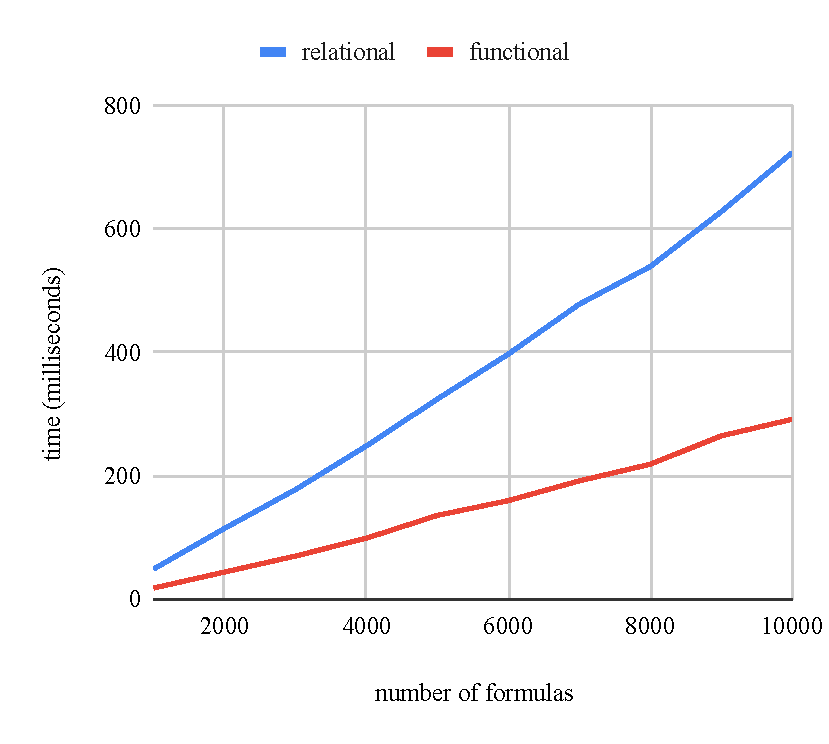
\includegraphics[height=0.85\textheight]{figures/propIOI.pdf}
  \end{center}
\end{frame}


\begin{frame}[fragile]
  \frametitle{Multiplication: \lstinline[basicstyle=\Large]{mulo n 10 q}}
  \begin{center}
    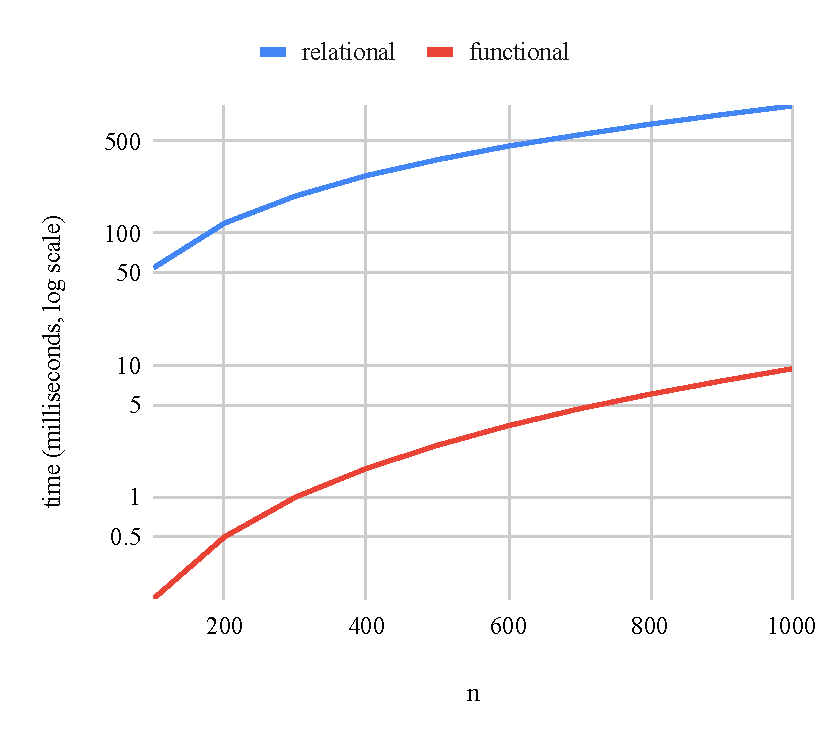
\includegraphics[height=0.85\textheight]{figures/muloIIO.pdf}
  \end{center}
\end{frame}


\begin{frame}[fragile]
  \frametitle{Division: \lstinline[basicstyle=\Large]{mulo (n/10) q n}}
  \begin{center}
    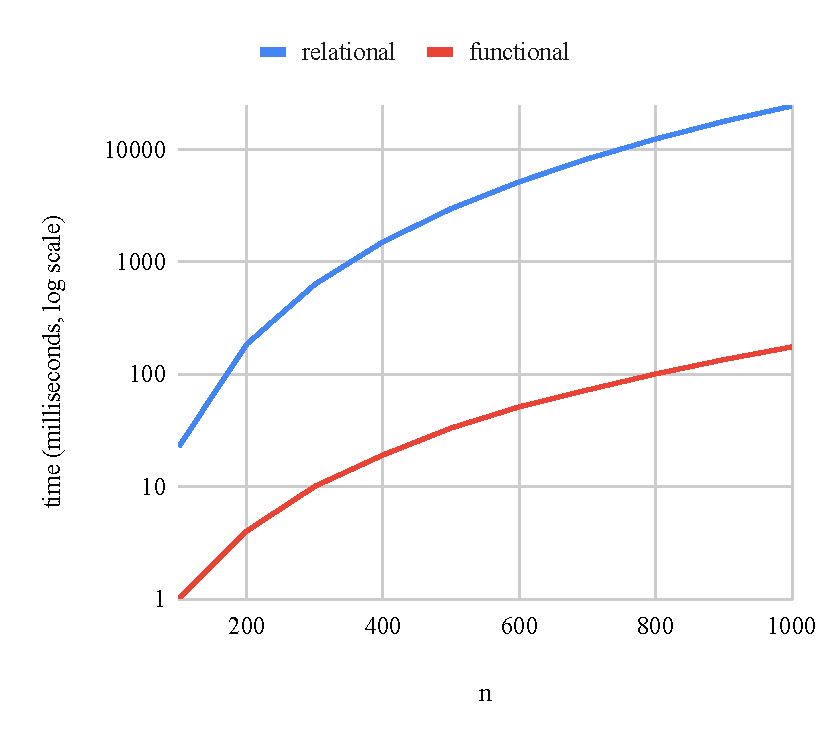
\includegraphics[height=0.85\textheight]{figures/muloIOI.pdf}
  \end{center}
\end{frame}


\begin{frame}[fragile]
  \frametitle{Multiplication Generation: \lstinline[basicstyle=\Large]{take n (mulo 10 q r)}}
  \begin{center}
    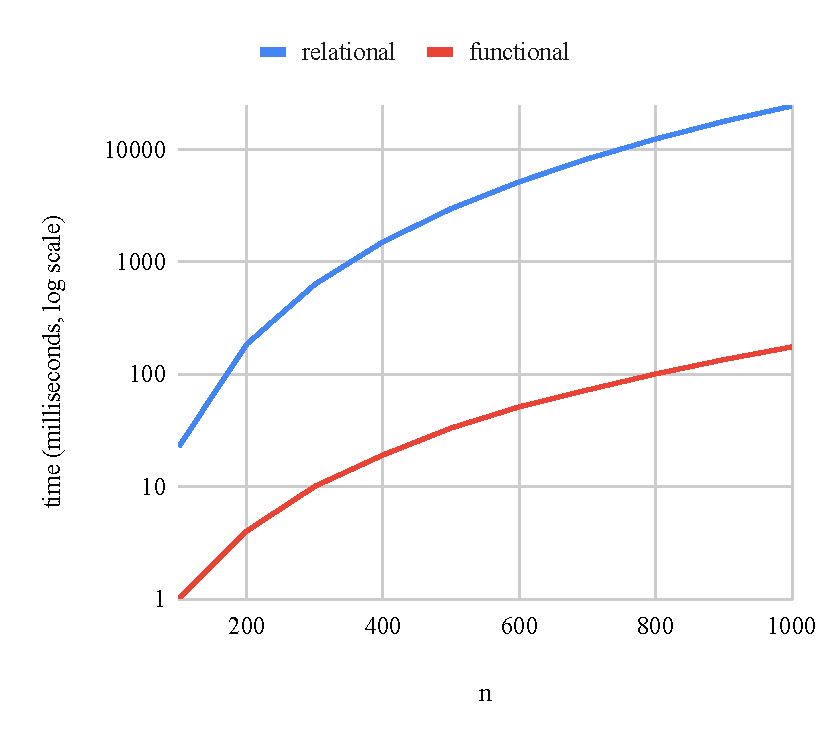
\includegraphics[height=0.85\textheight]{figures/muloIOI.pdf}
  \end{center}
\end{frame}

\begin{frame}[fragile]
  \frametitle{Data Types}
We generate weird data type declarations:
\begin{figure}[!t]
  \centering
  \begin{minipage}{\columnwidth}
    \begin{lstlisting}[label={add},
                      %  caption={Addition relation},
                       captionpos=b,
                       frame=tb]
type term =
  | Conj of (term* term)
  | Cons of (term* term)
  | Disj of (term* term)
  | Falso
  | Neg of term
  | Succ of term
  | Trueo
  | Var of term
  | Zero
        \end{lstlisting}
  \end{minipage}
\end{figure}

\begin{figure}[!t]
  \centering
  \begin{minipage}{\columnwidth}
    \begin{lstlisting}[label={add},
                      %  caption={Addition relation},
                       captionpos=b,
                       frame=tb]
elem$^o$ i st v =
  fresh (h t i') conde [
    (i === Zero /\ st === Cons (v, t));
    (i === Succ i' /\ st === Cons (h, t) /\ elem$^o$ i' t v)]
      \end{lstlisting}
  \end{minipage}
\end{figure}
\end{frame}

\begin{frame}[fragile]
  \frametitle{Need for Determinism Check: \lstinline[basicstyle=\Large]{mulo q 10 1000}}
  \begin{center}
    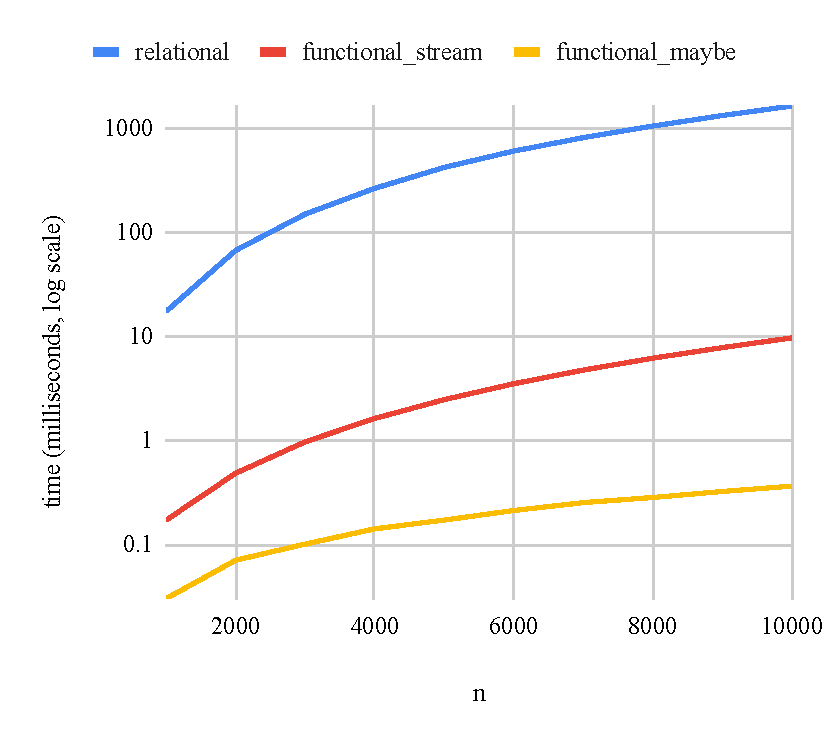
\includegraphics[height=0.85\textheight]{figures/maybe.pdf}
  \end{center}
\end{frame}

\begin{frame}[fragile]
  \frametitle{Need for Determinism Check}
  \begin{itemize}
    \item Replacing Stream with Maybe improves performance about 10 times for relations on natural numbers
    \item Functional (no monad) version is still faster
    \item Use determinism check to figure out when replacing Stream is feasible
    \item How to combine different monads naturally?
  \end{itemize}
\end{frame}

\begin{frame}[fragile]
  \frametitle{Need for Partial deduction}

\begin{center}
\mk can run a verifier backwards to get solver
\end{center}

\begin{center}
\begin{minipage}{0.3\textwidth}
  \lstinline{run q (eval$^o$ q true)}
\end{minipage}

\begin{center}
  Augmenting functional conversion with partial deduction must be beneficial
\end{center}
\end{center}


\end{frame}


\begin{frame}[fragile]
  \frametitle{Conclusion}
Conclusion
  \begin{itemize}
    \item We presented a functional conversion scheme as a series of examples
    \item The conversion speeds up implementations considerably
    \item We implemented the conversion scheme in Haskell
    \item Found some way to order conjuncts
  \end{itemize}

\vfill

Future work
  \begin{itemize}
    \item Integration with partial deduction
    \item Integration into a relational interpreters for solving framework
  \end{itemize}
\end{frame}



\end{document}
